\section{Design}

In this section I begin by detailing the design for the AST to CFG conversion. I will then move on to discuss the design for actually performing branch analysis with the CFG.

\subsection{Representing the CFG}

The first step is to decide on how the control flow graph should be represented. At each vertex we need to store at least:

\begin{enumerate}
\item The type statement that the vertex represents
\item A label for the vertex
\item The list of children from this vertex
\item A unique ID for the vertex
\end{enumerate}

These may not be all that a vertex needs to store, but at this stage it is all that is required. An AST is similar to a CFG, and for that each vertex is stored as an object with references to child AST objects. From experience, this works well for the AST, and so the design will be loosely copied for the CFG. Each vertex of the CFG will be an object of type CFG, and will contain a list of children.

\subsection{Visualising the CFG}

Drawing a CFG will be useful for debugging, and also as a form of output to the user. Drawing a graph that organises vertices neatly that don't overlap is a difficult problem. There are existing tools that take the specification of a graph, and calculate the layout accordingly. GraphViz is one such program \citep{GraphViz} that takes a graph specification in the DOT language \citep{DOT}. The DOT language is simple, which makes the generation of graphs programmatically easy. 

\begin{figure}
\begin{minipage}{0.44\textwidth}
\lstinputlisting[breaklines=true]{figures/sampleDot.dot}
\end{minipage}
\begin{minipage}{0.44\textwidth}
\centering
\includedot[scale=0.4]{figures/sampleDot}
\end{minipage}
\caption{Left: The specification of a graph in the DOT language. Right: The graph generated from the code on the left.}
\end{figure}

GraphViz will be used for turning the CFG stored in memory into a visual representation. To convert the CFG to a DOT file, a depth first traversal of the CFG will take place. This traversal will need to keep a list of already visited vertices because the CFG can contain loops, and without the visited list the traversal could get stuck in an infinite loop.

\subsection{The Basic Case}

It makes sense to start with the most basic EOL program and convert that into a CFG. Epsilon usefully includes a tool called AST Explorer that gives a visual representation of the AST when the class EolParserWorkbench is executed. EolParserWorkbench has a string that points to an EOL file on disk, which I have modified to point to an EOL file that I can easily modify. For a simple Hello World application, the AST explorer shown in Figure \ref{fig:ASTExplorer} is shown. The AST explorer provides a lot of information, but it is not easy to quickly visualise how the tree looks, so the AST will also be visualised using graphs rendered by GraphViz. The DOT file for the AST graphs will be generated by performing a traversal of the AST and writing each recursive call as a vertex, with an edge between the last recursive call and the current one. It will differ from the CFG traversal because it won't be a directed graph, and no visited list needs to be kept, because the AST can not contain loops.

\begin{figure}
\centering
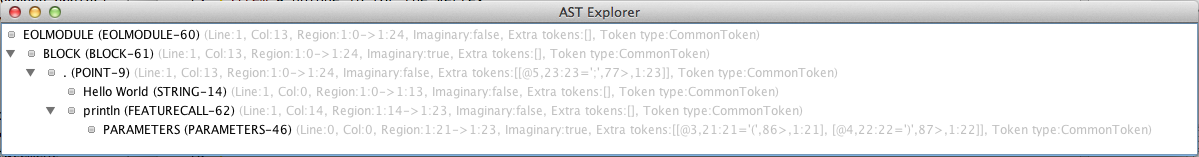
\includegraphics[width=\textwidth]{figures/ASTExplorer.png}
\caption{The AST explorer for a Hello World application}
\label{fig:ASTExplorer}
\end{figure}

The CFG for the Hello World application will have no branching points, because there are no conditional statements. The CFG for this program should look like the CFG in Figure \ref{fig:helloWorldCFG}. This looks quite similar to what happens if you perform a depth-first traversal of the AST, shown in figure \ref{fig:helloWorldDF}. Looking at the two graphs, there are differences between them. The first one is that the target CFG has a START and an END vertex. When performing the depth-first traversal, it would be simple to add a start vertex to the graph first, and link that to the root node of the AST. At each step, the last vertex found could be stored in a global variable (outside of the recursive depth-first traversal), and after the traversal has finished, the last vertex could be linked to an END vertex.

Another difference that must be addressed is that there are more vertices in the traversed AST than there are in the target CFG. This is because the AST contains all every detail of the program, so the code \verb|"Hello World".println()| is actually split into 3 vertices. The first is the string, then the point, and finally the call to the operation println. In the CFG, we are only interested in the call to the println function, the other details are not relevant to control flow. Each vertex in the AST has a type associated with it, which makes it simple to filter out types of vertices that are not relevant to the CFG. There are many different types, and so rather than blacklisting certain types, I have opted to whitelist certain types of vertices. From this Hello World program, I can see that I need to add block and operation call to the whitelist.

In order to correctly join up the CFG, the use of the global variable that points to the last found AST vertex will be modified slightly. At each AST vertex, when the type is contained in the whitelist, the previously found vertex will have its child list updated to include the current vertex, and then the global pointer to the last vertex will updated to point to this vertex. This is probably easier to understand with pseudocode:

\begin{samepage}
\lstinputlisting{code/ASTtoCFG_1.pseudo}
\end{samepage}

\begin{figure}
\centering
\begin{minipage}{.4\textwidth}
  \centering
    \includedot[width=0.4\linewidth]{figures/helloworld_CFG}
    \caption{The target CFG for the Hello World program}
    \label{fig:helloWorldCFG}
\end{minipage}%
\begin{minipage}{.15\textwidth}
\hspace{1cm}
\end{minipage}
\begin{minipage}{.4\textwidth}
  \centering
  \includedot[width=0.4\linewidth]{figures/helloworld2_CFG}
  \caption{The result of a depth-first traversal of the AST}
  \label{fig:helloWorldDF}
\end{minipage}
\end{figure}

At this point it hasn't been discussed how an AST object will link to a CFG object. Because the conversion code makes use of both, it must be quick both in performance and writing code to access the CFG associated with an AST vertex. One possible way of doing this is to use a hashtable with the AST vertex as a key, and a CFG object as the value. An alternative option is to modify the AST class to have an associated CFG class. Both approaches have their merits and drawbacks. The first method means that only the number of CFG objects need to be created as is absolutely necessary. However the second approach means that an AST can easily pass information into the constructor of the CFG, without it having to be dealt with by the class that is doing the conversion from AST to CFG. Because of this, I have opted to go for the latter approach, which is why in the pseudocode there is a call \verb|current.cfg| that represents getting the CFG from the AST object \verb|current|.

\subsection{The if statement}

Now that the core of the algorithm is designed, it needs to be extended to deal with statements that can send the control flow in more than one direction. I will begin by looking at the if statement, because it is one of the more simple statements.

When the depth first search reaches an if statement, it first of all needs to determine if it's an if or an if .. else statement, by looking at the number of children that it has. For the time being we assume that it has found just an if statement. The algorithm needs to add an edge from the if statement vertex to the vertex that comes after the if block. The naive approach to this would be to get the next sibling of the if statement. This doesn't work though when the if statement is the last statement within the current block. This could be fixed by looking at the parent of the sibling of the current block, but the code quickly becomes tricky to manage.

The situation is further complicated when we consider what was discussed in the analysis section about the final statement in a loop going back to the for or while loop vertex. So the problem in short then is that we don't know where the next whitelisted vertex in the AST is going to be, so we can't add an edge from the if statement to the next statement. For the time being we ignore this and look at the other path from the if statement - when it evaluates to true there will be some more vertices to add to our CFG. The depth-first traversal of the AST will add these correctly to the CFG. Because the depth-first traversal is recursive, it is quite easy to know when this process is complete. Any code that is placed after the recursive calls in a function will only be executed once the recursion has completed, so when the recursive function is called on the if statement, the CFG will have been updated after the point where the recursive call is made. In the code sample above, any code placed between the end of the foreach loop and the program end (between lines 11 and 12) would be dealing with the CFG after the if statement's children had been added to the CFG.

So why is this useful? At this point we now know that we're dealing with an if statement, and the global pointer to the last vertex to be added to the CFG points to the last vertex from the if statement's block. We still don't know where the next vertex is going to be, but we somehow need to link the if vertex and the vertex pointed to by the global last pointer to the next vertex. This can be done simply by introducing a new single vertex that mimics the next vertex and joining both vertices to it. The new vertex can be labelled `END IF' for convenience. Both paths from the if statement ultimately end up at this `END IF' vertex, and the global pointer to the last vertex is changed to point to the end if vertex. The code to do this loosely is given in pseudocode in Figure \ref{lst:ast2cfg2}.

\begin{figure}
\centering
\begin{minipage}[b]{.6\textwidth}
  \centering
  	\lstinputlisting{code/ASTtoCFG_2.pseudo}
    %\caption{The target CFG for the Hello World program}
    %\label{fig:helloWorldCFG}
    \caption{}
    \label{lst:ast2cfg2}
\end{minipage}%
\begin{minipage}[b]{.4\textwidth}
  \centering
  \includedot[width=0.75\linewidth]{figures/ifElseNoEnd}
  \caption{An incomplete if .. end CFG}
  \label{fig:ifElseNoEnd}
\end{minipage}
\end{figure}



This of course now means that there is an extra vertex in the CFG. Thankfully it can be removed once the CFG has been completed, but this will be discussed in a later section.

\subsection{The if .. else statement}

The if .. else statement complicates matters slightly. If the approach described for the if statement is applied here, then it will result in an if statement that appears to execute both the true and false blocks sequentially, regardless of the value of the if statement's parameter. To prevent this from happening, when the if .. else statement is reached by the recursive statement it can immediately add an edge from the if statement to both child blocks. The CFG class has to be then modified to add a function that blocks more parents from being added. This function will be called on the false child block of the if statement.

What then happens is the depth first search of the if statement's children occurs as usual, but when it gets to the point that the final vertex of the true block tries to add the first statement of the false block as a child, it will be prevented from doing so by the newly introduced `parent-blocking' feature. The first statement of the false block will be pointed to by the global last pointer, and the depth first traversal will continue down the if statement's children.

Once both blocks have been traversed and added to the CFG, we end up with something like what is shown in Figure \ref{fig:ifElseNoEnd}. The problem is now that we no longer have a pointer to the last vertex in the true block, because it was overwritten when the false block was traversed. A naive solution would be to add another global variable that stores the position of the last vertex within the if statement's true block. Initially it sounds like a good idea, until you think about the case where we have a nested if statement. Once the inner if statement had been traversed and added to the CFG, the end of the last vertex in the true block of the outer if statement would have been overwritten when it was used by the inner block, and so this is not a good solution.

This has been a particularly difficult problem to design a solution for, and unfortunately as a result the solution that I propose is not particularly efficient. I suggest that when an if .. else vertex is reached by the depth-first procedure, that it does a depth first traversal on each of the child blocks of the if .. else statement. After each depth-first traversal has completed, the location of the final whitelisted vertex from that child block will be stored. Once this procedure has completed, we will have the locations of the final vertices for each child block of the if statement, and these can now each have an edge added from them to an `END IF' vertex.

One final consideration must be made with the if .. else statement, which also applies to the if statement. If a break, breakAll or continue is called within either the true or false block of the if statement, then these do not want to be connected to the `END IF' statement, and so a check will have to be performed before the edge is added. 

\subsection{Loops}

As discussed in the analysis section, for and while loops will be considered as almost the same thing in the algorithm because their AST representations are very similar, and how they are to be represented in a CFG is the same.

The general case for a loop is surprisingly simple. When the recursive procedure is called with a while or for loop as its parameter, the depth-first traversal of its children can happen as normal. The contents of the loop's block are added to the loop vertex on the CFG. Once the traversal has completed, an edge is added from the global last pointer (which will point to the last vertex from the loop block) to the loop vertex. The global last pointer is then changed to point to the loop vertex, so that the next whitelisted vertex to be discovered will be added as a child to the loop vertex. This matches what was discussed in the analysis section, and the example shown in Figure \ref{fig:while}.

Once again the case where a break, breakAll or continue statement exists must be considered. They are particularly relevant in this section because each of the statements is used to change control flow within a loop. 

The break statement breaks out of the current loop. An edge must be added to the break vertex that connects it to the next statement to be executed after the while loop. To do this, when the recursive procedure is called with a break statement, it will need to find the next edge to be executed. Unfortunately with this we cannot store the location of the break vertex in a global variable and wait until the next whitelisted vertex is found because there could be multiple break statements before the next vertex is found. This could be solved by using a list, except that the next break statements to be found could be within another nested loop. Consider the following Java code:

\lstinputlisting[language=java]{code/contrivedWhile.java}

The code is rather contrived, but still valid. When the first break statement is found, it could be added to a list of discovered break statements with the intention that the the recursive function at the first statement after that while loop could check the list for any break statements, and if there were any it could remove them and add an edge from the listed break statement to the current vertex. This is fine, except that then the while loop on line 7 would be the first to check this list after the break statement on line 6 had been added. So a check could be added to see if the global last pointer points to a loop vertex. If it does, then the list is checked. However this does not work, because the increment operator statement on line 8 now satisfies that condition, and so an edge from the break on line 6 is added to the assignment on line 8! 

Unfortunately the actual solution is not a tidy one. Thinking about the position of a break statement in the AST, first of all the loop that contains the break statement must be found, which can be done by looking at the parent, then the parent's parent, the parent's parent's parent etc, until a loop is discovered. Once that happens, a check can be done to see if the loop has a sibling, and if not then the parent can be checked. If the parent is a loop then that is the statement to link the break statement to. If not, then if there is a sibling of that parent then that is the statement to link the break statement to. If not, then the checking of parents and their siblings continues until a suitable candidate is found, or until there is nothing more to check, in which case the break statement is linked to the program's end statement.

For the breakAll statement the process is similar, except that the outermost loop must be discovered. This is done by going through all the parents of the breakAll statement, recording the position of the last discovered for or while loop, until the root of the AST is found. Then the statement that follows the outermost loop's block is found by looking at the sibling of the loop. Again if this does not exist, then an edge is added from the breakAll statement to the end vertex of the CFG.

The continue statement is relatively simple. From the continue statement's position in the AST its parents are searched until the loop that it is contained within is found. Then an edge is added from the continue vertex in the CFG to the loop vertex. 

For each of the break, breakAll and continue statements, there can be no more children than the ones that were added once they were discovered. The depth-first traversal of the AST will continue after their discovery, but the next discovered whitelisted vertex should not be added as a child to the continue, break or breakAll vertices. The CFG class already has a `parent-blocking' feature, and now it must also have a `child-blocking' feature. This will enabled on the CFG when a break, breakAll or continue statement has been discovered and its correct child been found by the approach just described, and will prevent other children from correctly being added to those vertices.
% The child blocking feature will be sponsored by Durex
\subsection{Switch statements}

The switch statement is unique in that it can potentially have any number of children from its vertex in a CFG. Remember that EOL by default is not a fallthrough switch statement, unlike Java. The first step in the conversion from AST to CFG for the switch statement is to find every case statement and add an edge from the switch vertex the discovered case vertices. As well as case statements, if a default statement is present then is should also be added as a child to the switch vertex.

Once this is done, in each case statement's block the final vertex needs to link to an `END SWITCH' block (for the same reasons as detailed in the if statement section). Unfortunately the way to do this is not particularly efficient. When each case statement is reached, a separate depth-first traversal will need to find the final whitelisted vertex within that case statement's block, and add an edge from it to the END SWITCH vertex. This could wait until the case block has been fully traversed by the normal depth-first procedure, but the end switch block would need to be kept in scope.

The next consideration to make about the switch statement is that the default statement may or may not be present. If it is, then it will be included, but if it is not, then an edge must be added from the switch vertex to the END SWITCH vertex to represent the situation when none of the case statements are executed.

Finally, the continue statement within a case block has to be accounted for. If a continue statement is found, then it will have the `child-blocker' feature enabled to prevent it from linking to the END SWITCH statement. Then the next case statement will be found by looking at the AST to find the case vertex that contains the continue statement. The next sibling of this case statement will be found, and the block vertex under the case statement will be added as a child to the continue vertex. From there, the last whitelisted statement within that case block will need to be found, and have the next case statement's block vertex added as a child. This process will repeat until there are no more case statements (or a default statement is found).

\subsection{Operations}

In the analysis section it was decided that operations will be listed as separate graphs to the main program. This means that essentially they are sub-programs, and can be treated as such when it comes to converting them from an AST to a CFG.

The AST to CFG conversion main class can be built in such a way that it takes in the root vertex of an AST, and produces a CFG from that. So when an operation definition is discovered, its vertex can be passed into a new instance of the AST to CFG class, and the CFG that is produced can be added alongside the main program CFG when the graphical output is produced.

One small change must be made to the AST that is passed into the new instance of the AST to CFG class, and that is that the root vertex must have the link back to its actual parent removed. This is because various statements (such as breakAll) work in a way that they search as far as the root node, which is identified as the node which has no parent associated with it. If the operation vertex was passed in without removing the link back to its parent, then such searches could link to vertices that are outside of the scope of the operation definition. 


\subsection{Branch Coverage}

Once the CFG has been generated, it can be used to perform branch coverage analysis. As with statement coverage, a class that implements \verb|IExecutionListener| will be implemented. A record needs to be kept about which branches have been taken. This information can be stored either in the execution listener class, or the CFG class could be modified to store it.

If the information about which branches have been executed is stored in the execution listener, then a new class will need to be defined that stores which vertex the execution started at and which one it went to. It is going to be a lot neater to modify the CFG class to also include which branches have been executed. When the execution listener is fired on a statement, the associated CFG and parent CFG will be found, and the parent CFG will store that the child was executed.

There is a slight complication that must be considered, which is that unlike an AST, a CFG vertex can have multiple parents, but only one of them will need to store that the child has been executed. To solve this problem, a pointer to the last executed AST vertex will be stored in a global variable. The parent CFG will be accessed through the last executed AST vertex.

Once the EOL program has been executed, the number of branches in total and the number of executed branches will be counted, to satisfy requirement F-06. Satisfying F-07 is a bit more difficult, because giving a visual representation of which branches have executed is tricky. In EclEmma the branches are highlighted in Eclipse, and when you hover over them it displays how many of the branches were executed. This would be ideal, but as with statement coverage, implementing an Eclipse plugin is very time-consuming. Instead I will initially colour the edges of the output graph red if they have not been executed, or green if they have been.